\documentclass[a4paper,oneside,openright,11pt]{report}

\usepackage{amsmath}
\usepackage{amssymb}
\usepackage{amsthm}
\usepackage[labelfont=bf,labelsep=period]{caption}
\usepackage{enumitem}
\usepackage{float}
\usepackage[margin=2.5cm]{geometry}
\usepackage{graphicx}
\usepackage{numbertabbing}
\usepackage{times}
\usepackage{url}
\usepackage{xspace}
\usepackage{hyperref}
\usepackage{cleveref}

\floatstyle{ruled}
\newfloat{algo}{htbp}{algo}
\floatname{algo}{Algorithm}

%%% fill in your data here %%%
\newcommand{\reporttitle}{Optimistic rollups: Offchain Labs Arbitrum}
\newcommand{\reportauthor}{Marius Asadauskas}
\newcommand{\reportauthororigin}{Bern, Switzerland}
\newcommand{\reportleiter}{Prof.\ Christian Cachin}
\newcommand{\reporturl}{http://crypto.unibe.ch/}
\newcommand{\reportsubtitle}{Cost differences analysed}
\newcommand{\reportdate}{23. December 2021}


\begin{document}

\pagenumbering{roman}

\begin{titlepage}  
  \thispagestyle{empty}

  \begin{center}  
    \begin{figure}[t]  
      \center{
\includegraphics[scale=0.5]{UNI_Bern.png}}
      \vspace{1in}     
    \end{figure}
    
    {\bfseries\Huge \reporttitle \\[2mm]
      \Large \reportsubtitle}\\
    \vspace{1.5cm}

    {\bfseries\LARGE Seminar report}\\
    \vspace{1.5cm}
    
    {\Large \reportauthor\\[2mm]
      from\\[2mm]
      \reportauthororigin}\\
    \vspace{1.5cm}

    {\Large Faculty of Science, University of Bern}\\
    \vspace{1.5cm}

    {\Large \reportdate}\\
    \vspace{1.5cm}

    \vspace*{\fill}
    {\Large
      \reportleiter\\
      Cryptology and Data Security Group\\
      Institute of Computer Science\\
      University of Bern, Switzerland\\}
  \end{center}
\end{titlepage}


\chapter*{\centering Abstract}
\begin{quote}\noindent
  The recent growth in popularity surrounding blockchain-based technologies has brought many
  new users into the world of cryptocurrencies. While the increase in user base is mostly regarded 
  as positive, it has also brought many of the issues related to distributed systems to light. One of 
  these issues being the limited throughput that various cryptocurrencies suffer from.
  This effect is especially noticeable in Ethereum, where the transaction costs have
  increased drastically as a result.
  
  To mitigate this issue, Layer 2 solutions have been proposed. These would offload and process
  some of the transaction data offchain and only post the most important information on chain.
  The most prominent of these layer 2 solutions is Arbitrum~\cite{l2Beat} with their protocol 
  being based on optimistic rollups.
  
  In the following report, we will analyse the cost differences between transactions happening on 
  the layer 1 Ethereum blockchain and transactions happening on layer 2 via Arbitrum.
\end{quote}

\tableofcontents

\pagenumbering{arabic}

\chapter{Introduction}
\label{ch:intro}

\section{Transaction Fees}
Transaction fees exist inside cryptocurrencies to act as an incentive for miners to add a transaction to a block.
This incentive is necessary since before adding a transaction to a block, you must first perform validity 
checks, such as making sure that no double spending is happening. You must also perform other 
computations, such as computing the Merkel root of the transaction and updating the Merkel tree. 
Without an incentive to do so, a miner could instead focus all their resources on winning the Proof of
Work race without wasting any resources.

Furthermore, the idea of transaction fees is nothing new. It was first proposed in the 
Bitcoin Witepaper~\cite{nakamoto2008bitcoin} by Satoshi Nakamoto and is still in use
today. Problems only start to arise once the throughput limit of the network has been reached. 
Once that happens, users stop paying for the computational costs and instead pay a much higher fee
to get a spot in the block. 
As a result, transaction costs rise in tandem with the popularity of a cryptocurrency.

\section{Layers in Blockchains}
In the blockchain ecosystem, Layer 1 is the term used when describing the underlying blockchain architecture.
The term Layer 2 is used when talking about protocols that run on top of Layer 1 and do not require
modifications to the first layer. An example of a Layer 1 protocol would be the Ethereum blockchain. 
An example of a layer 2 protocol would be Arbitrum, which runs on top of the Ethereum blockchain. 
You can see this illustrated below in~\cref{fig:Layer1_Layer2_comparison}.

\begin{figure}
	\centering
	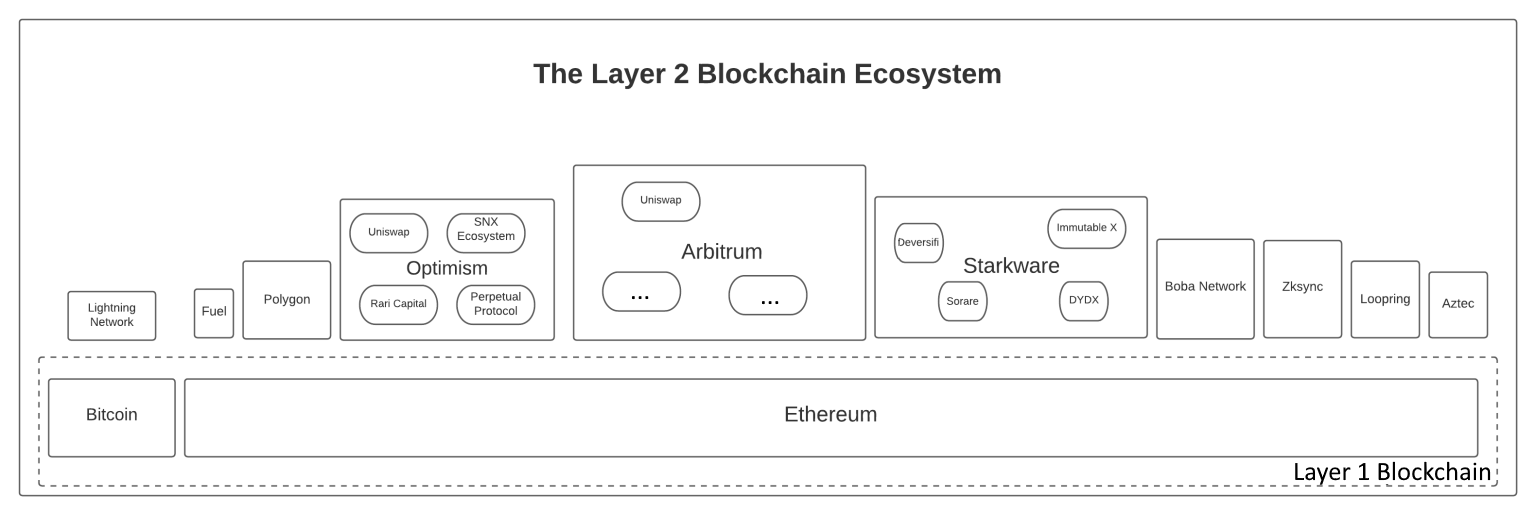
\includegraphics[scale=0.8]{./Pictures/Layer-2-Ecosystem-Map.png}
	\caption{Layer differentiation}
	\label{fig:Layer1_Layer2_comparison}
\end{figure}

\section{Optimistic Rollups}
We already mentioned Arbitrum and how it is a possible solution for Ethereum's throughput problem
but, we have yet to mention how it functions. Arbitrum uses a protocol based on optimistic rollups.
The name optimistic rollups itself is made up of two parts.
\subsection{Rollups}
The rollup half of optimistic rollups refers to the fact that only a rollup of the transaction data
gets posted on Layer 1. For example if you create a smart contract in Arbitrum you only have 
to post it's hash and some other parameters on Layer 1. Doing so takes up much less storage 
on the Ethereum blockchain and having the 256-bit cryptographic hash on the blockchain still 
ensures that the smart contract is immutable.

\subsection{Optimistic}
The optimistic part refers to the process of how the rollups get posted on chain. 
Namely any manager of a smart contract can claim a state change. Arbitrum is optimistic in
the sense that if nobody rejects the claim the hash gets updated. If however in the timeframe
of a week someone were to object to the claim, only then does arbitrum verify its validity.

\begin{figure}[h]
	\centering
	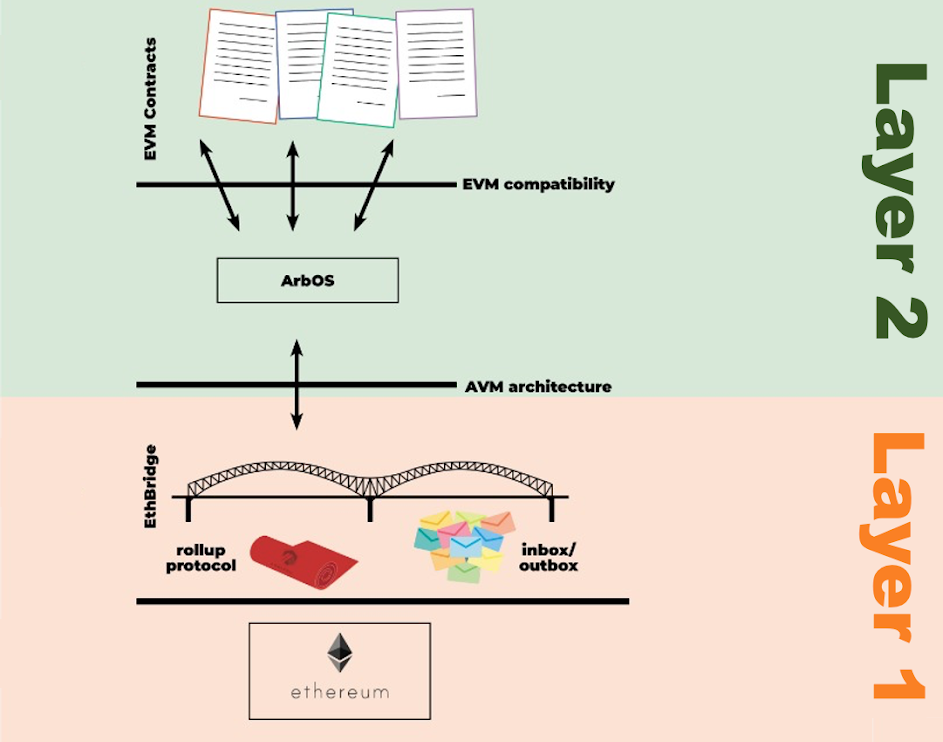
\includegraphics[scale=0.5]{./Pictures/Optimistic-Rollup.png}
	\caption{Optimistic Rollups}
	\label{fig:Optimistic_Rollups}
\end{figure}
  
\chapter{Background}

\section{Arbitrum White Paper}
The Arbitrum White paper~\cite{ArbWP} was the first paper to propose optimistic rollups back in 2018. 
Over the years many of the details surrounding Arbitrum's implementation have changed and been refined. 
In 2018 the main focus of Arbitrum was to increase privacy, scalability, and computational power of smart
contracts. Nowadays the word privacy appears nowhere on Arbitrum's website or in the protocol description. 
Enhanced computational power still remains a priority but the main focus has shifted to scalability and 
increasing throughput. The main idea of relying on optimistic rollups to achieve this goal however
remains unchanged.

\section{Arbitrum Developers Guide}
The Arbitrum developers guide~\cite{ArbDevGuide} is the main source of information 
for when it comes to Arbitrum today. It contains instructions on how to deploy smart 
contracts on Arbitrum. Information on how transaction fees are calculated. Descriptions 
on what smart contracts running on Ethereum make Arbitrum possible. 
Most if not all information related to Arbitrum today can be found there.

\section{Arbiscan}
Arbiscan is a website~\cite{Arbiscan} which allows its users to explore the Arbitrum 
blockchain without having to download the chain locally. This interface makes 
gathering data from the Arbitrum chain much easier and was the main tool we used 
when calculating the average transaction costs in Arbitrum.
The website is controlled by Arbitrum and was made together with the help of the 
Etherscan team~\cite{ArbEthScan}.

\chapter{Analysing the cost differences}
In the following section we will be analysing the cost differences between Arbitrum and Ethereum
from both a theoretical and a practical point of view.

\section{Theoretical costs}
For finding out the theoretical cost differences between Arbitrum and Ethereum our best reference was
the Arbitrum developer guide~\cite{ArbDevGuide}. This contained detailed explanations on how Arbitrum
calculates the cost of each transaction.

Similar to Ethereum, Arbitrum uses a measure called Arb. Gas. The idea behind Arb. Gas is 
identical to that of Ethereum. Since nodes have to verify a transaction, you pay them
in Arb. Gas. The only difference is that Arb. Gas costs much less than Ethereum Gas and has
a higher global limit. Translating Arb. Gas into Ether also works similarly. You take the 
Arb. Gas value and multiply it with the base fee per Gas unit. This Fee is an estimate
of the Ethereum gas fee. So we define
\[
	P := \text{Expected L1 Gas Price}
\]

For each transaction on Arbitrum you pay in four areas:
\begin{itemize}
  \item L2 \textit{tx}: A base fee for each L2 transaction, to cover the cost of servicing a transaction
  \[
		\text{L2 } \textit{tx} = \frac{CP}{B}.
	\] 
	With $C$ being the L1 cost for an aggregator to submit a Batch to L1 and $B$ being the batch size.
	
  \item L1 \textit{calldata}: A fee per units of L1 calldata directly attributable to the transaction 
  (each non-zero byte of calldata is 16 units, and each zero byte of calldata is 4 units)
  \[
		\text{L1 } \textit{calldata} = P \cdot \text{calldata units}.
	\]
	
  \item \textit{computation}: A fee per unit of ArbGas used by the transaction.
  \[
		\textit{computation} = \text{Arb Gas} \cdot \text{Base Price}
	\]
  With the Base Price bing determined by the congestion of a network. If the Arbitrum network is under heavy load
  the base price gets multiplied by $9/8$. If the network is under low load, the base price gets multiplied by $7/8$.
  Furthermore, The base price cannot go below $P/10'000$.
  
  \item \textit{storage}: A fee per location of EVM contract storage, based on the net increase in EVM storage due to the transaction.
  \[
		\textit{storage} = 2000 \cdot P \cdot \text{storage}
	\]
	You must pay 2'000 times the estimated L1 gas price per 256-Bit word of storage allocated. 
	Considering that in Ethereum you pay 20'000 gas per 256-bit word this implies that you pay 10\% 
	the expected Ethereum price.
\end{itemize}

If we add it all together
\[
	\text{total} = \text{L2 } \textit{tx} + \text{L1 } \textit{calldata} + \textit{computation} + \textit{storage}
\]
Furthermore if we assume that the base price is the minimum value, we get
\[
	\text{total} = P(\frac{C}{B} + \text{calldata units} + \frac{\text{Arb. Gas}}{10'000} + 2000 \cdot \text{storage})
\]

\subsection{Example: Simple transaction}
	For a simple transaction from one address to another on Ethereum you would have to pay 21'000 gas,
	according to the Ethereum yellow paper~\cite{wood2014ethereum}.
	If we assume that the base fee is estimated correctly and no tip was given, we would get
	\[
		\text{Eth. cost} = 21,000 \cdot (\text{Base Fee} + \text{tip}) = 21'000 \cdot P.
	\]
	The same transaction on Arbitrum would cost us
	\[
		\text{Arb. cost} = P(\frac{C}{B} + 0 + 2000 \cdot 0 + \frac{21'000}{10'000}) = \frac{CP}{B} + 2.1P.
	\]
	We can already see that the main cost comes from submitting the transaction to the L1 chain, while verifying the
	transaction would only cost us 2.1 gas.
	If we take some reasonable values we would get $C = 1'200'000, B = 200$ 
	and then the Cost becomes
	\[
		\text{Arb.cost} \approx 6'000 P + 2.1 P = 6002.1 P 
	\]
	So in theory a basic Arbitrum transaction could cost around $6002.1/21'000 \approx 0.286$, 28.6\% the price of
	an Ethereum transaction. However this value depends heavily on $\frac{C}{B}$ and the percentage will
	only go down the more difficult a transaction becomes. Consider the following
	\[
		\lim_{\text{Gas} \to \infty} \frac{P(6'000 + \text{Gas}/10'000)}{P \cdot \text{Gas}} = 
		\lim_{\text{Gas} \to \infty} \frac{6000 + \text{Gas}/10'000}{\text{Gas}} =
		\lim_{\text{Gas} \to \infty} \frac{6000}{\text{Gas}} + \frac{1}{10'000} =
		\frac{1}{10'000}
	\]
\section{Practical costs}
On the 31st of august 2021 the Arbitrum Mainnet went online~\cite{ArbMainNet} 
and became accessible to the public. This development allowed us to not only theoretically 
analyse the cost differences but also analyse the practical cost differences between 
transactions happening on Arbitrum and transactions happening on Ethereum.

A motivation to do so was the fact that average transaction costs were readily available for 
Ethereum~\cite{EthTxCost}, while for Arbitrum there were no such services.
Furthermore, Arbiscan, the main blockchain explorer for Arbitrum, is made 
with the help of Etherscan~\cite{ArbEthScan} and both applications are close to identical in terms
of design and functionality. One of the key differences between the two sites being that Etherscan 
provides this information while Arbiscan does not. The exclusion of the average transaction costs
seems intentional from the side of Arbitrum.

\subsection{Data Gathering}
	Arbiscan provides an API for developers to gather and request data from the blockchain. 
	This was very helpful since it meant that we did not have to store the blockchain ourselves.
	Using the provided API seemed like the most logical way of gathering data. 
	However, the provided API calls were for very specific 
	requests that involved exact account addresses and not for the type of broad requests we needed 
	to calculate average transaction costs.
	
	We instead opted to get the data ourselves from the Arbiscan website directly via html extraction.
	For this we employed the use of urllib3~\cite{UrlLib3}, which would request and store the pages and 
	BeautifulSoup~\cite{BS}, which was responsible for extracting the information.
	The Site contains a blockchain
	history of the past 500'000 Transactions with 50 transactions a page and this amounts to around 2 weeks. 
	
	\subsection{Average calculation}
	Arbiscan stores a total of 10'000 pages with 50 transactions each. This amounts to around
	2 weeks worth of transaction data. Instead of processing all 10'000 pages and putting a large
	load on the Arbiscan servers we opted to process a limited amount of pages distributed 
	over the entire set. However, taking pages at random was also not an option. This would only 
	give us the average of 50 entries. We instead would create cluster of multiple pages and 
	distribute theses clusters evenly throughout the 10'000 pages.
	Using urllib we collected the data, parsed it and then used the function 
	\textbf{numpy.mean(}costs\textbf{)} to get the average of each page and the average of
	each cluster. The function \textbf{numpy.meadian(}costs\textbf{)}, would be more robust
	to outliers but it would return the median value instead of an average value.
	
	Plotting this in matplotlib would give us the average transaction fees over the course of the backlog.
	\begin{figure}[h]
		\centering
		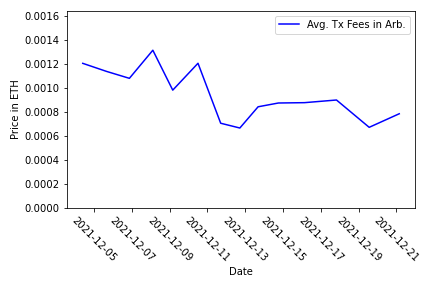
\includegraphics[scale=0.8]{./Pictures/arb_avg_eth.png}
		\label{fig:Average_Arbitrum_Ether_Fees}
	\end{figure}
	
	Furthermore, using a python module to get historic Ethereum prices would allow us to plot the average
	transaction price in dollars. For this we used the python module cryptocompare. Multiplying the costs
	with the Ether prices at the given dates gave us the following graph
	
	\begin{figure}[h]
		\centering
		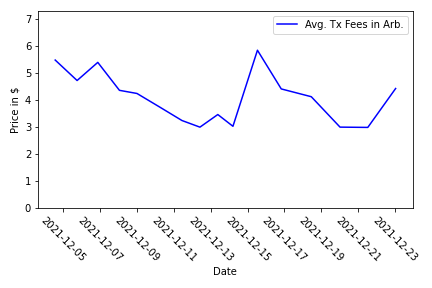
\includegraphics[scale=0.8]{./Pictures/arb_avg_usd.png}
		\label{fig:Average_Arbitrum_USD_Fees}
	\end{figure}
	
	\subsection{Comparison}
	To compare the average Arbitrum transaction fees with the given Ethereum transaction fees required us
	to first find a source of Ethereum transaction fees for given dates. For this we downloaded a csv file from
	a website~\cite{ETHFees} which only included Layer 1 transactions in the average calculation. Comparing the
	data to our chart we got the following results.
	
	\begin{figure}[h]
		\centering
		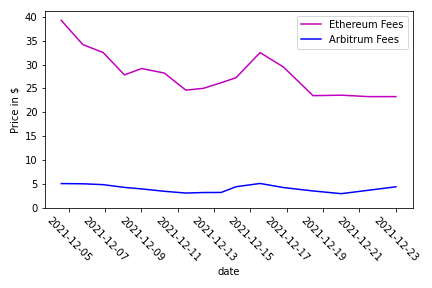
\includegraphics[scale=0.8]{./Pictures/arb_eth_fees.png}
		\label{fig:Arbitrum_Ethereum_Fees}
	\end{figure}
	

\chapter{Conclusion}
\label{ch:conclusion}

This report set out to give a clear comparison and provide concrete numbers 
between transactions on layer 1, that happen on the
Ethereum blockchain and transactions on layer 2, which happen on Arbitrum.
For this we had to extract data from the Arbitrum blockchain and calculate the 
average transaction fees ourselves, since the Arbitrum blockchain explorer refused to provide this data. 

When comparing both averages directly with each other we can see that the cost of the 
average transaction is not much lower on the Arbitrum network. 
At times it even exceeds the transaction costs on the Ethereum blockchain itself.
For this reason we probably cannot see the average transaction fees on Arbiscan.

This however does not mean that one shouldn't use the Arbitrum network.
If everyone went back to the Ethereum chain the throughput would decrease and
also the transaction fees would go up.
What could help these fees go down is more users switching to the Arbitrum network and
making the transaction fees for the Ethereum chain smaller.

The only shady thing is that Arbiscan does not display the average transaction fees although 
this data is readily available to them. It highlights the strong centralization of Arbitrum and the
power they hold over the network. Restricting the flow of unfavourable information and instead only
showing favourable information.

% The bibliography appears after any appendix.

% using BiBTeX is required
\bibliography{Report}

% any bibstyle is fine, this one give particularly compact output 
\bibliographystyle{ieeetran}
\end{document}
